\fenicschapter{Common and Unusual Finite Elements}
              {Common and Unusual Finite Elements}
              {Robert C. Kirby, Anders Logg and Andy R. Terrel}
              {kirby-6}

\newcommand{\elemententry}[1]{\null

\includegraphics[width=2.5cm]{#1}}

This chapter provides a glimpse of the considerable range of finite
elements in the literature and the challenges that may be involved
with automating ``all'' the elements. Many of the elements presented
here are included in the FEniCS project already; some are future work.

%------------------------------------------------------------------------------
\section{Ciarlet's Finite Element Definition}

As discussed in Chapter~\ref{chap:kirby-7}, a finite element is defined by a
triple $(K, \mathcal{P}_K, \mathcal{L}_K)$, where
\begin{itemize}
\item
  $K \subset \R^d$ is a bounded closed subset of $\R^d$ with nonempty
  interior and piecewise smooth boundary;
\item
  $\mathcal{P}_K$ is a function space on $K$ of dimension $n_K < \infty$;
\item
  $\mathcal{L}_K = \{\ell^K_1, \ell^K_2, \ldots, \ell^K_{n_K}\}$ is a
  basis for $\mathcal{P}_K'$ (the bounded linear functionals on
  $\mathcal{P}_K$).
\end{itemize}

This definition was first introduced by Ciarlet in a set of lecture
notes~\cite{Ciarlet1975} and became popular after his 1978
book~\cite{Ciarlet1978,Ciarlet2002}. It remains the standard
definition today, see for example~\cite{BrennerScott2008}. Similar
ideas were introduced earlier in~\cite{CiarletRaviart1972} which
discusses unisolvence of a set of interpolation points~$\Sigma =
\{a_i\}_i$. This is closely related to the unisolvence of~$\mathcal{L}_K$. In fact, the set of
functionals~$\mathcal{L}_K$ is given by $\ell^K_i(v) = v(a_i)$. It is
also interesting to note that the Ciarlet triple was originally
written as~$(K,P,\Sigma)$ with $\Sigma$
denoting~$\mathcal{L}_K$. Conditions for uniquely determining a
polynomial based on interpolation of function values and derivatives
at a set of points was also discussed in~\cite{BrambleZlamal1970},
although the term unisolvence was not used.

%------------------------------------------------------------------------------
\section{Notation}

It is common to refer to the space of linear
functionals~$\mathcal{L}_K$ as the \emph{degrees of freedom} of the
element~$(K, \mathcal{P}_K, \mathcal{L}_K)$. The degrees of freedom
are typically given by point evaluation or moments of function values
or derivatives. Other commonly used degrees of freedom are point
evaluation or moments of certain components of function values, such
as normal or tangential components, but also directional derivatives.
We summarize the notation used to indicate degrees of freedom
graphically in Figure~\ref{fig:notation}. A filled circle at a point
$\bar{x}$ denotes point evaluation at that point,
\begin{displaymath}
  \ell(v) = v(\bar{x}).
\end{displaymath}
We note that for a vector valued function~$v$ with~$d$ components, a
filled circle denotes evaluation of all components and thus
corresponds to~$d$ degrees of freedom,
\begin{displaymath}
  \begin{split}
    \ell_1(v) &= v_1(\bar{x}), \\
    \ell_2(v) &= v_2(\bar{x}), \\
    \ell_3(v) &= v_3(\bar{x}).
  \end{split}
\end{displaymath}
An arrow denotes evaluation of a component of a function value in a
given direction, such as a normal component $\ell(v) = v(\bar{x})
\cdot n$ or tangential component $\ell(v) = v(\bar{x})
\cdot t$. A plain circle denotes evaluation of all first derivatives,
a line denotes evaluation of a directional first derivative such as a
normal derivative $\ell(v) = \nabla v(\bar{x}) \cdot n$.  A dotted
circle denotes evaluation of all second derivatives. Finally, a circle
with a number indicates a number of interior moments (integration
against functions over the domain~$K$).

\begin{figure}[h]
  %\psfrag{v}{\emph{point evaluation}}
  %\psfrag{vn}{\emph{point evaluation of directional component}}
  %\psfrag{dv}{\emph{point evaluation of all first derivatives}}
  %\psfrag{dvn}{\emph{point evaluation of directional derivative}}
  %\psfrag{d2v}{\emph{point evaluation of all second derivatives}}
  %\psfrag{int}{\emph{interior moments}}
  \hspace{2cm}
  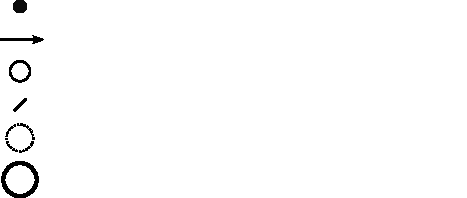
\includegraphics[width=4.5cm]{chapters/kirby-6/pdf/notation.pdf}
  \caption{Notation}
  \label{fig:notation}
\end{figure}

\newpage

%------------------------------------------------------------------------------
\section{The Argyris Element}

\subsection{Definition}

The Argyris triangle~\cite{ArgyrisFriedScharpf1968,Ciarlet2002} is based
on the space \(
\mathcal{P}_K = P_5(K) \) of quintic
polynomials over some triangle \( K \).  It can be pieced together
with full \( C^1 \) continuity between elements with \( C^2 \)
continuity at the vertices of a triangulation. Quintic polynomials in
$\R^2$ are a 21-dimensional space, and the dual basis \( \mathcal{L}_K
\) consists of six degrees of freedom per vertex and one per each edge. The vertex
degrees of freedom are the function value, two first derivatives to specify the
gradient, and three second derivatives to specify the unique
components of the (symmetric) Hessian matrix.

\begin{figure}[h]
  \begin{center}
    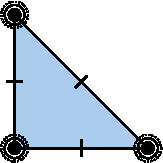
\includegraphics[width=\smallfig]{chapters/kirby-6/pdf/ARG5.pdf}
    \caption{The quintic Argyris triangle.}
  \end{center}
\end{figure}

\subsection{Historical notes}

The Argyris element~\cite{ArgyrisFriedScharpf1968} was first called the
TUBA element and was applied to fourth-order plate-bending problems.
In fact, as Ciarlet points out~\cite{Ciarlet2002}, the element also
appeared in an earlier work by Felippa~\cite{Felippa1966}.

The normal derivatives in the dual basis for the Argyris element
prevent it from being affine-interpolation equivalent. This prevents
the nodal basis from being constructed on a reference cell and
affinely mapped. Recent work by Dominguez and
Sayas~\cite{DominguezSayas2008} has developed a transformation that
corrects this issue and requires less computational effort than
directly forming the basis on each cell in a mesh.

The Argyris element can be generalized to polynomial degrees higher
than quintic, still giving \( C^1 \) continuity with \( C^2 \)
continuity at the vertices~\cite{vSolinSegethDolevzel2004}. The Argyris
element also makes an appearance in exact sequences of finite
elements, where differential complexes are used to explain the
stability of many kinds of finite elements and derive new
ones~\cite{ArnoldFalkWinther2006}.

\newpage

%------------------------------------------------------------------------------
\section{The Brezzi--Douglas--Marini element}

\subsection{Definition}

The Brezzi--Douglas--Marini element~\cite{BrezziDouglasMarini1985}
discretizes \( H(\mathrm{div}) \). That is, it provides a vector field
that may be assembled with continuous normal components so that global
divergences are well-defined.  The BDM space on a simplex in \( d \)
dimensions (\( d=2,3 \)) consists of vectors of length \( d \) whose
components are polynomials of degree \( q \) for
\( q \geq 1 \).

\begin{figure}[h]
  \begin{center}
    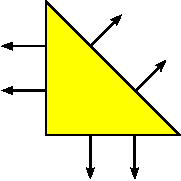
\includegraphics[width=\smallfig]{chapters/kirby-6/pdf/BDM1.pdf}
    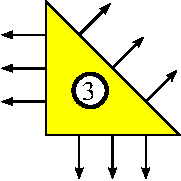
\includegraphics[width=\smallfig]{chapters/kirby-6/pdf/BDM2.pdf}
    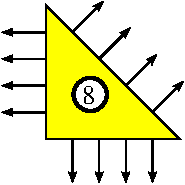
\includegraphics[width=\smallfig]{chapters/kirby-6/pdf/BDM3.pdf}
    \caption{The linear, quadratic and cubic Brezzi--Douglas--Marini
      triangles.}
  \end{center}
\end{figure}

The degrees of freedom for the BDM triangle include the normal component on each
edge, specified either by integral moments against $P_q$ or the value
of the normal component at
\( q + 1 \) points per edge.
For \( q > 1 \), the degrees of freedom also include integration
against gradients of $P_q(K)$ over $K$.  For \( q > 2 \), the degrees
of freedom also include integration against curls of $b_K P_{q-2}(K)$
over $K$, where \( b_K \) is the cubic bubble function associated with
\( K \).

\authornote{What about tets? Will also make up for the empty space on the next page.}

The BDM element is also defined on rectangles and boxes, although it
has quite a different flavor. Unusually for rectangular domains, it is
not defined using tensor products of one-dimensional polynomials, but
instead by supplementing polynomials of complete degree \( [P_q(K)]^d
\) with extra functions to make the divergence onto \( P_q(K) \).  The
boundary degrees of freedom are similar to the simplicial case, but
the internal degrees of freedom are integral moments against \(
[P_q(K)]^d \).

\subsection{Historical notes}

The BDM element was originally derived in two
dimensions~\cite{BrezziDouglasMarini1985} as an alternative to the
Raviart--Thomas element using a complete polynomial space. Extensions
to tetrahedra came via the ``second-kind'' elements of
\nedelec{}~\cite{Nedelec1986} as well as in Brezzi and
Fortin~\cite{BrezziFortin1991}. While \nedelec{} uses quite different
internal degrees of freedom (integral moments against the
Raviart--Thomas spaces), the degrees of freedom in Brezzi and Fortin
are quite similar to~\cite{BrezziDouglasMarini1985}.

A slight modification of the BDM element constrains the normal
components on the boundary to be of degree \( q - 1 \) rather than \(
q \). This is called the Brezzi--Douglas--Fortin--Marini or BDFM
element~\cite{BrezziFortin1991}. In similar spirit, elements with
differing orders on the boundary suitable for varying the polynomial
degree between triangles were derived
in~\cite{BrezziDouglasMarini1985a}.  Besides mixed formulations of
second-order scalar elliptic equations, the BDM element also appears
in elasticity~\cite{ArnoldFalkWinther2007a}, where it is seen that each
row of the stress tensor may be approximated in a BDM space with the
symmetry of the stress tensor imposed weakly.

\authornote{Fill up the blank space here. Adding a discussion and possibly a figure for tets should help.}

\newpage

%------------------------------------------------------------------------------
\section{The Crouzeix--Raviart element}

\subsection{Definition}

The Crouzeix--Raviart element~\cite{CrouzeixRaviart1973} most commonly
refers to a linear non-confor\-ming element. It uses piecewise linear
polynomials, but unlike the Lagrange element, the degrees of freedom
are located at edge midpoints rather than at vertices.  This gives
rise to a weaker form of continuity, but it is still a suitable
$C^0$-nonconforming element. The extension to tetrahedra in $\R^3$
replaces the degrees of freedom on edge midpoints by degrees of
freedom on face midpoints.

\authornote{What other element does it refer to? Sounds like there may be several, but I just know about this one.}

\begin{figure}[h]
  \begin{center} 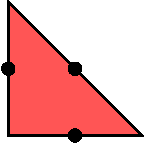
\includegraphics[width=\smallfig]{chapters/kirby-6/pdf/CR1.pdf}
    \caption{The linear Crouzeix--Raviart triangle.}  \end{center}
\end{figure}

\subsection{Historical notes}

Crouzeix and Raviart developed two simple Stokes elements, both using
pointwise evaluation for degrees of freedom. The second element used
extra bubble functions to enrich the typical Lagrange element, but the
work of Crouzeix and Falk~\cite{CrouzeixFalk1989} later showed that
the bubble functions were in fact not necessary for quadratic and
higher orders.

\authornote{The discussion in the previous paragraph should be expanded
so it states more explicitly what this has to do with the CR element.}

The element is usually associated with solving the Stokes problem but
has been used for linear elasticity~\cite{HansboLarson2003} and
Reissner–-Mindlin plates~\cite{ArnoldFalk1989} as a remedy for
locking. There is an odd order extension of the element from Arnold
and Falk.

\authornote{Missing reference here to odd order extension.}

\newpage

%------------------------------------------------------------------------------
\section{The Hermite Element}

\subsection{Definition}

The Hermite element~\cite{Ciarlet2002} generalizes the classic cubic
Hermite interpolating polynomials on the line segment. On the
triangle, the space of cubic polynomials is ten-dimensional, and the
ten degrees of freedom are point evaluation at the triangle vertices
and barycenter, together with the components of the gradient evaluated
at the vertices. The generalization to tetrahedra is analagous.

\begin{figure}[h]
  \begin{center}
    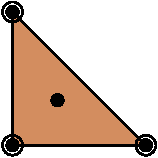
\includegraphics[width=\smallfig]{chapters/kirby-6/pdf/HER3.pdf}
    \caption{The cubic Hermite triangle.}
  \end{center}
\end{figure}

Unlike the cubic Hermite functions on a line segment, the cubic
Hermite triangle and tetrahedron cannot be patched together in a fully
\( C^1 \) fashion.

\subsection{Historical notes}

Hermite-type elements appear in the finite element literature almost
from the beginning, appearing at least as early as the classic paper
of Ciarlet and Raviart~\cite{CiarletRaviart1972}. They have long been
known as useful \( C^1 \)-nonconforming
elements~\cite{Braess2007,Ciarlet2002}.  Under affine mapping, the
Hermite elements form
\emph{affine-interpolation equivalent} families.~\cite{BrennerScott2008}.

\newpage

%------------------------------------------------------------------------------
\section{The Lagrange Element}

\subsection{Definition}

The best-known and most widely used finite element is the Lagrange
$P_1$ element. In general, the Lagrange element uses \( \mathcal{P}_K
= P_q(K) \), polynomials of degree $q$ on $K$, and the degrees of
freedom are simply pointwise evaluation at an array of points. While
numerical conditioning and interpolation properties can be
dramatically improved by choosing these points in a clever
way~\cite{missing}, for the purposes of this chapter the points may be
assumed to lie on an equispaced lattice.

\authornote{Missing reference for statement about node placement.}

%\begin{figure}[h]
%  \begin{center}
%    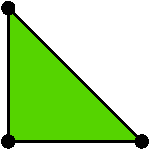
\includegraphics[width=\smallfig]{chapters/kirby-6/pdf/P1.pdf}
%    \caption{The linear Lagrange (Courant) triangle).}
%  \end{center}
%\end{figure}

\begin{figure}[h]
  \begin{center}
    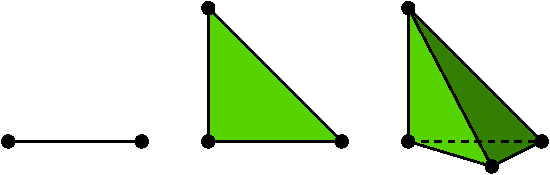
\includegraphics[width=15cm]{chapters/kirby-6/pdf/P1-1d2d3d.pdf}
    \caption{The linear Lagrange interval, triangle and tetrahedron.}
  \end{center}
\end{figure}

\begin{figure}[h]
  \begin{center}
    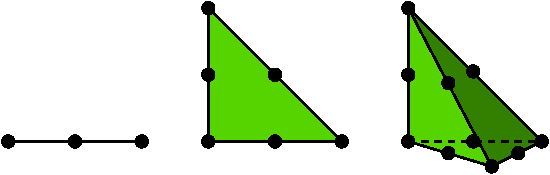
\includegraphics[width=15cm]{chapters/kirby-6/pdf/P2-1d2d3d.pdf}
    \caption{The quadratic Lagrange interval, triangle and tetrahedron.}
  \end{center}
\end{figure}

\begin{figure}[h]
  \begin{center}
    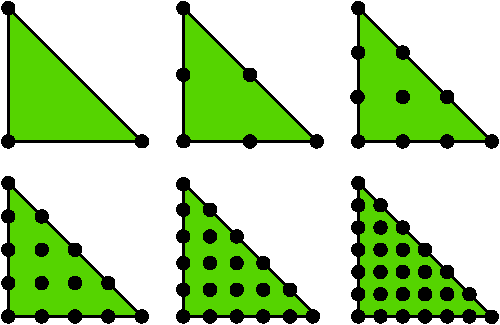
\includegraphics[width=15cm]{chapters/kirby-6/pdf/P1-6.pdf}
    \caption{The Lagrange $P_q$ triangle for $q = 1,2,3,4,5,6$.}
  \end{center}
\end{figure}

\subsection{Historical notes}

Reams could be filled with all the uses of the Lagrange elements.  The
Lagrange element predates the modern study of finite elements.  The
lowest-order triangle is sometimes called the \emph{Courant} triangle,
after the seminal paper~\cite{Courant1943} in which variational
techniques are considered and the \( P_1 \) triangle is used to derive
a finite difference method. The rest is history.

\authornote{Expand the historical notes for the Lagrange element.
  As far as I can see, Bramble and Zlamal
  don't seem to be aware of the higher order Lagrange elements (only
  the Courant triangle). Their paper from 1970 focuses only on Hermite
  interpolation.}

\newpage

%------------------------------------------------------------------------------
\section{The Morley Element}

\subsection{Definition}

The Morley triangle~\cite{Morley1968} is a simple \( H^2
\)-nonconforming quadratic element that is used in fourth-order
problems.  The function space is simply \( \mathcal{P}_K = P_2(K) \),
the six-dimensional space of quadratics.  The degrees of freedom
consist of pointwise evaluation at each vertex and the normal
derivative at each edge midpoint. It is interesting that the Morley
triangle is neither \( C^1 \) nor even \( C^0 \), yet it is suitable
for fourth-order problems, and is the simplest known element for this
purpose.

\begin{figure}[h]
  \begin{center}
    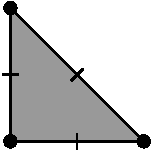
\includegraphics[width=\smallfig]{chapters/kirby-6/pdf/MOR2.pdf}
    \caption{The quadratic Morley triangle.}
  \end{center}
\end{figure}

\subsection{Historical notes}

The Morley element was first introduced to the engineering literature
by Morley in 1968~\cite{Morley1968}. In the mathematical literature,
Lascaux and Lesaint~\cite{LascauxLesaint1975} considered it in the
context of the patch test in a study of plate-bending elements.

\authornote{Fill up page.}

\newpage

%------------------------------------------------------------------------------
\section{The \nedelec{} Element}

\subsection{Definition}

The widely celebrated \( H(\mathrm{curl}) \)-conforming elements of
\nedelec{}~\cite{Nedelec1980,Nedelec1986} are much used in electromagnetic
calculations and stand as a premier example of the power of
``nonstandard'' (meaning not lowest-order Lagrange) finite elements.

\begin{figure}[h]
  \begin{center}
    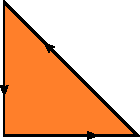
\includegraphics[width=\smallfig]{chapters/kirby-6/pdf/NED1.pdf}
    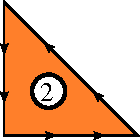
\includegraphics[width=\smallfig]{chapters/kirby-6/pdf/NED2.pdf}
    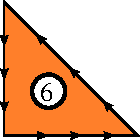
\includegraphics[width=\smallfig]{chapters/kirby-6/pdf/NED3.pdf}
    \caption{The linear, quadratic and cubic \nedelec{} triangles.}
  \end{center}
\end{figure}

On triangles, the function space~$\mathcal{P}_K$ may be obtained by a
simple rotation of the Raviart--Thomas basis functions, but the
construction of the tetrahedral element is substantially different. In
the lowest order case \( q = 1 \), the space \( \mathcal{P}_K \) may
be written as functions of the form
\[
v(x) = \alpha + \beta \times x,
\]
where \( \alpha \) and \( \beta \) are vectors in \( \R^3 \).  Hence,
$\mathcal{P}_K$ contains all vector-valued constant functions and some
but not all linears. In the higher order case, the function space may
be written as the direct sum
\[
\mathcal{P}_K = [P_{q-1}(K)]^3 \oplus S_q,
\]
where
\[
S_q = \{ v \in [\tilde{P}_q(K)]^3 : v \cdot x = 0 \}.
\]
Here, \( \tilde{P}_q(K) \) is the space of homogeneous polynomials of
degree \( q \) on $K$. An alternate characterization of
$\mathcal{P}_K$ is that it is the space of polynomials of degree \( q
+ 1 \) on which the $q$th power of the elastic stress tensor
vanishes. The dimension of $\mathcal{P}_q$ is exactly
\begin{displaymath}
  n_K = \frac{q(q+2)(q+3)}{2}.
\end{displaymath}

\authornote{What is the $q$th power of the elastic stress tensor?}

\authornote{What is the dimension on triangles?}

The degrees of freedom are chosen to ensure tangential continuity
between elements and thus a well-defined global curl. In the lowest
order case, the six degrees of freedom are the average value of the
tangential component along each edge of the tetrahedron, hence the
term ``edge elements''.  In the more general case, the degrees of
freedom are the \( q-1 \) tangential moments along each edge, moments
of the tangential components against \( (P_{q-2})^2 \) on each face,
and moments against \( (P_{q-3})^3 \) in the interior of the
tetrahedron.

For tetrahedra, there also exists another family of elements known as
Nedelec elements of the second kind, appearing in~\cite{Nedelec1986}.
These have a simpler function space at the expense of more complicated
degrees of freedom.  The second kind space of order \( q \) is simply
vectors of polynomials of degree \( q \). The degrees of freedom are
integral moments of degree \( q \) along each edge together with
integral moments against lower-order first-kind bases on the faces and
interior.

\authornote{Note different numbering compared to RT, starting at 1,
  not zero.}

\subsection{Historical notes}

\nedelec{}'s original paper~\cite{Nedelec1980} provided rectangular and
simplicial elements for \( H(\mathrm{div}) \) and \( H(\mathrm{curl})
\) based on incomplete function spaces.  This built on earlier
two-dimensional work for Maxwell's
equations~\cite{AdamGourdinNedelecEtAl1980} and extended the work of Raviart
and Thomas for \( H(\mathrm{div}) \) to three dimensions. The second
kind elements, appearing in~\cite{Nedelec1986}, extend the
Brezzi--Douglas--Marini triangle~\cite{BrezziDouglasMarini1985} to three
dimensions and curl-conforming spaces. We summarize the relation
between the Nedelec elements of first and second kind with the
Raviart--Thomas and Brezzi--Douglas--Marini elements in
Table~\ref{tab:nedelecelements}.

\linespread{1.5}
\begin{table}
  \begin{center}
    \begin{tabular}{|c||c|c|}
      \hline
      Simplex & $\Hdiv$ & $\Hcurl$ \\
      \hline \hline
      $K \subset \R^2$
      &
      \begin{tabular}{p{4.5cm}p{1.5cm}}
        $\mathrm{RT}_{q-1}$   & $\mathcal{P}_{q}^{-} \Lambda^1(K)$ \\
        $\mathrm{BDM}_q$  & $\mathcal{P}_{q} \Lambda^1(K)$ \\
      \end{tabular}
      &
      \begin{tabular}{p{2.5cm}p{1.5cm}}
        $\mathrm{NED}_{q-1}(\mathrm{curl})$ & --- \\
        &
      \end{tabular}
      \\ \hline
      $K \subset \R^3$
      &
      \begin{tabular}{p{4.5cm}p{1.5cm}}
        $\mathrm{RT}_{q-1} = \mathrm{NED}^1_{q-1}(\mathrm{div})$  & $\mathcal{P}_{q}^{-} \Lambda^2 (K)$ \\
        $\mathrm{BDM}_q = \mathrm{NED}^2_q(\mathrm{div})$ & $\mathcal{P}_{q} \Lambda^2(K)$ \\
      \end{tabular}
      &
      \begin{tabular}{p{2.5cm}p{1.5cm}}
        $\mathrm{NED}^1_{q-1}(\mathrm{curl}) $ & $\mathcal{P}_{q}^- \Lambda^1 (K)$ \\
        $\mathrm{NED}^2_q(\mathrm{curl})$ & $\mathcal{P}_{q} \Lambda^1 (K)$
      \end{tabular}
      \\ \hline
    \end{tabular}
    \linespread{1.0}
    \caption{Nedelec elements of the first and second kind and their
      relation to the Raviart--Thomas and Brezzi--Douglas--Marini
      elements as well as to the notation of finite element exterior calculus.}
    \label{tab:nedelecelements}
  \end{center}
\end{table}
\linespread{1.0}

In many ways, \nedelec{}'s work anticipates the recently introduced
finite element exterior calculus~\cite{ArnoldFalkWinther2006}, where the
first kind spaces appear as \( \mathcal{P}_q^-\Lambda^k \) spaces and
the second kind as \(
\mathcal{P}_q\Lambda^k \). Moreover, the use of a differential
operator (the elastic strain) in~\cite{Nedelec1980} to characterize
the function space foreshadows the use of differential
complexes~\cite{ArnoldFalkWinther2006}.

\authornote{Should we change the numbering of the Nedelec elements and
  Raviart--Thomas elements to start at $q = 1$?}

\newpage

%------------------------------------------------------------------------------
\section{The PEERS Element}

\subsection{Definition}

The PEERS element~\cite{ArnoldBrezzi1974aDouglas1984} provides a stable tensor
space for discretizing stress in two-dimensional mixed elasticity
problems. The stress tensor \( \sigma \) is represented as a \( 2
\times 2 \) matrix, each row of which is discretized with a
vector-valued finite element.  Normally, one expects the stress tensor
to be symmetric, although the PEERS element works with a variational
formulation that enforces this condition weakly.

The PEERS element is based on the Raviart--Thomas element described in
Section~\ref{sec:raviartthomas}.  If \( \mathrm{RT}_0(K) \) is the
lowest-order Raviart-Thomas function space on a triangle \( K \) and
\( b_K \) is the cubic bubble function that vanishes on \( \partial K
\), then the function space for the PEERS element is given by
\begin{displaymath}
\mathcal{P}_K = \left[\mathrm{RT}_0(K) \oplus \mathrm{span}\{\mathrm{curl}( b_K )\} \right]^2.
\end{displaymath}

\begin{figure}[h]
  \begin{center}
    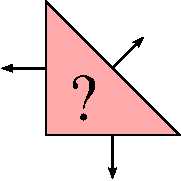
\includegraphics[width=\smallfig]{chapters/kirby-6/pdf/PEERS.pdf}
    \caption{The PEERS triangle. One vector-valued component is shown.}
  \end{center}
\end{figure}

\authornote{Which degrees of freedom in the interior? The curl?}

\authornote{Is this really an element? We could also introduce other
  mixed elements like Taylor--Hood. But perhaps it's suitable to
  include it since it is not a trivial combination of existing
  elements (the extra curl part).}

\subsection{Historical notes}

Discretizing the mixed form of planar elasticity is quite a difficult
task.  Polynomial spaces of symmetric tensors providing inf-sup
stability are quite rare, only appearing in the last
decade~\cite{ArnoldWinther2002}. A common technique is to relax the
symmetry requirement of the tensor, imposing it weakly in a
variational formulation.  This extended variational form requires the
introduction of a new field discretizing the assymetric portion of the
stress tensor.  When the PEERS element is used for the stress, the
displacement is discretized in the space of piecewise constants, and
the asymmetric part is discretized in the standard space of continuous
piecewise linear elements.

The PEERS element was introduced in~\cite{ArnoldBrezzi1974aDouglas1984}, and
some practical details, including postprocessing and hybridization
strategies, are discussed in~\cite{ArnoldBrezzi1974a1985}.

\newpage

%------------------------------------------------------------------------------
\section{The Raviart--Thomas Element}
\label{sec:raviartthomas}

\subsection{Definition}

The Raviart--Thomas element, like the Brezzi--Douglas--Marini and
Brezzi--Douglas--Fortin--Marini elements, is an \( H(\mathrm{div})
\)-conforming element.  The space of order~$q$ is constructed to be
the smallest polynomial space such that the divergence maps \(
\mathrm{RT}_q(K) \) onto \( P_q(K) \). The function space
$\mathcal{P}_K$ is given by
\begin{displaymath}
  \mathcal{P}_K = P_{q-1}(K) + x P_{q-1}(K).
\end{displaymath}
The lowest order Raviart--Thomas space thus consists of vector-valued
functions of the form
\begin{displaymath}
  v(x) = \alpha + \beta x,
\end{displaymath}
where $\alpha$ is a vector-valued constant and $\beta$ is a scalar
constant.

On triangles, the degrees of freedom are the moments of the normal
component up to degree \( q \), or, alternatively, the normal
component at \( q + 1 \) points per edge. For higher order spaces,
these degrees of freedom are supplemented with integrals against a
basis for \( [P_{q-1}(K)]^2 \).

\begin{figure}[h]
  \begin{center}
    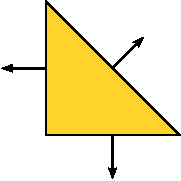
\includegraphics[width=\smallfig]{chapters/kirby-6/pdf/RT0.pdf}
    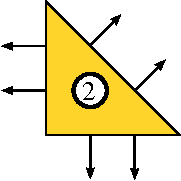
\includegraphics[width=\smallfig]{chapters/kirby-6/pdf/RT1.pdf}
    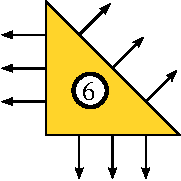
\includegraphics[width=\smallfig]{chapters/kirby-6/pdf/RT2.pdf}
    \caption{The zeroth order, linear and quadratic Raviart--Thomas
      triangles.}
  \end{center}
\end{figure}

\subsection{Historical notes}

The Raviart--Thomas element was introduced in~\cite{RaviartThomas1977}
in the late 1970's, the first element to discretize the mixed form of
second order elliptic equations. Shortly thereafter, it was extended
to tetrahedra and boxes by \nedelec{}~\cite{Nedelec1980} and so is
sometimes referred to as the Raviart--Thomas--\nedelec{} element or a
first kind $\Hdiv$ element.

On rectangles and boxes, there is a natural relation between the
lowest order Raviart--Thomas element and cell-centered finite
differences. This was explored in~\cite{RussellWheeler1983}, where a
special quadrature rule was used to diagonalize the mass matrix and
eliminate the flux unknowns. Similar techniques are known for
triangles~\cite{ArbogastDawsonKeenanEtAl1998}, although the stencils are
more complicated.

\newpage

%------------------------------------------------------------------------------
\section{Summary}

\begin{center}
  \begin{longtable}{|p{1.7cm}|p{4.7cm}|p{2.5cm}|p{1.5cm}|p{2cm}|}
    \hline
    Notation & Element family  & $\mathcal{L}_K$ & $\mathrm{dim} \, \mathcal{P}_K$ & References \\
    \hline
    \hline
    %------------------------------------------------------------------------
    $\mathrm{ARG}_5$ & Quintic Argyris &
    \elemententry{chapters/kirby-6/pdf/ARG5.pdf} &
    $21$ & \\
    \hline
    %------------------------------------------------------------------------
    $\mathrm{BDM}_1$ & Brezzi--Douglas--Marini &
    \elemententry{chapters/kirby-6/pdf/BDM1.pdf} &
    $6$ & \\
    \hline
    %------------------------------------------------------------------------
    $\mathrm{BDM}_2$ & Brezzi--Douglas--Marini &
    \elemententry{chapters/kirby-6/pdf/BDM2.pdf} &
    $12$ & \\
    \hline
    %------------------------------------------------------------------------
    $\mathrm{BDM}_3$ & Brezzi--Douglas--Marini &
    \elemententry{chapters/kirby-6/pdf/BDM3.pdf} &
    $20$ & \\
    \hline
    %------------------------------------------------------------------------
    $\mathrm{CR}_1$ & Crouzeix--Raviart &
    \elemententry{chapters/kirby-6/pdf/CR1.pdf} &
    $3$ & \\
    \hline
    %------------------------------------------------------------------------
    $\mathrm{HERM}_q$ & Hermite &
    \elemententry{chapters/kirby-6/pdf/HER3.pdf} &
    $10$ & \\
    \hline
    %------------------------------------------------------------------------
    $P_1$ & Lagrange &
    \elemententry{chapters/kirby-6/pdf/P1.pdf} &
    $3$ & \\
    \hline
    %------------------------------------------------------------------------
    $P_2$ & Lagrange &
    \elemententry{chapters/kirby-6/pdf/P2.pdf} &
    $6$ & \\
    \hline
    %------------------------------------------------------------------------
    $P_3$ & Lagrange &
    \elemententry{chapters/kirby-6/pdf/P3.pdf} &
    $10$ & \\
    \hline
    %------------------------------------------------------------------------
    $\mathrm{MOR}_1$ & Morley &
    \elemententry{chapters/kirby-6/pdf/MOR2.pdf} &
    $6$ & \\
    \hline
    %------------------------------------------------------------------------
    $\mathrm{NED}_1$ & \nedelec{} &
    \elemententry{chapters/kirby-6/pdf/NED1.pdf} &
    $3$ & \\
    \hline
    %------------------------------------------------------------------------
    $\mathrm{NED}_2$ & \nedelec{} &
    \elemententry{chapters/kirby-6/pdf/NED2.pdf} &
    $8$ & \\
    \hline
    %------------------------------------------------------------------------
    $\mathrm{NED}_3$ & \nedelec{} &
    \elemententry{chapters/kirby-6/pdf/NED3.pdf} &
    $15$ & \\
    \hline
    %------------------------------------------------------------------------
    $\mathrm{PEERS}$ & PEERS &
    \elemententry{chapters/kirby-6/pdf/PEERS.pdf} &
    ? & \\
    \hline
    %------------------------------------------------------------------------
    $\mathrm{RT}_0$ & Raviart--Thomas &
    \elemententry{chapters/kirby-6/pdf/RT0.pdf} &
    $3$ & \\
    \hline
    %------------------------------------------------------------------------
    $\mathrm{RT}_0$ & Raviart--Thomas &
    \elemententry{chapters/kirby-6/pdf/RT1.pdf} &
    $8$ & \\
    \hline
    %------------------------------------------------------------------------
    $\mathrm{RT}_0$ & Raviart--Thomas &
    \elemententry{chapters/kirby-6/pdf/RT2.pdf} &
    $15$ & \\
    \hline
    %------------------------------------------------------------------------
  \end{longtable}
\end{center}

\newpage

\authornote{Add references to table.}

\authornote{Indicate which elements are supported by FIAT and SyFi.}

\authornote{Include formula for space dimension as function of $q$ for
  all elements.}
